\chapter{Схемы для многократного вовлечения регенерированного урана в топливный цикл}\label{ch:ch3}

% \chapter{2}
Далее будут представлены схемы, позволяющие решить поставленную в диссертационной работе задачу, отвечая всем сформулированным условиям для рассматриваемых составов регенерата, с различным исходным содержанием, что соответствует условиям многократного рецикла. Такие каскады позволяют добиться заданной цели возврата регенерата в топливный цикл -- одновременно выполнить ограничения на концентрации четных изотопов в продукте и обеспечить заданную пропорцию между исходным регенератом и продуктом.

Разрабатываемая схема каскада должна не только обеспечить выполнение требований по содержанию четных изотопов в продукте, но и израсходовать на производство низкообогащенного урана 100\% имеющегося в распоряжении регенерированного урана. Второе условие позволяет вернуть в топливный цикл весь выделенный из ОЯТ регенерат вне зависимости от его изотопного состава, что гарантирует возможность использования подобной схемы для обогащения неоднократно облученного регенерата урана.

\section{Схема двойного каскада с НОУ-разбавителем}

Развитием идеи двойного каскада является модификация в виде дополнительного использования в качестве разбавителя низкообогащенного урана, полученного из природного урана. Такая схема представлена на рис. \ref{p2left}. Принцип работы такой схемы опирается на идею <<пространственного>> разделения на легкую ($^{232,233,234}$U) и тяжелую фракции ($^{235,238}$U), предложенную в двойном каскаде, и заключается в следующем. 

\begin{figure}[ht]
    \centerfloat{
\includegraphics[scale=0.9]{cascades/p2left}}
    \caption{Схема модифицированного двойного каскада для обогащения регенерированного урана. Обозначения: $E$ -- поток регенерированного урана; $P_1$ -- поток отбора первого каскада, выступающий питанием второго каскада; $P_2$ -- поток отбора второго каскада; $W_1$ -- поток отвала первого каскада; $W_2$ -- поток тяжелой фракции (условный «отвал») второго каскада; $P_0$ -- поток НОУ-разбавителя; $P$ -- финальный продукт (товарный низкообогащенный уран (НОУ))}\label{p2left}
\end{figure}

В первом каскаде исходный материал обогащается по изотопам $^{232,233,234,235,236}$U, а во втором каскаде смесь делится на две фракции, так, чтобы в тяжелой фракции сконцентрировался продукт с пониженным содержанием $^{232,233,234}$U по отношению к питающей второй каскад смеси. Таким образом, в первом каскаде, на одном из концов, смесь обогащают по легким изотопы (в первую очередь $^{232,233,234,235}$U) в потоке $P_1$. Концентрацию $^{235}$U можно варьировать, однако целесообразно сохранять в диапазоне 5–20\%. Верхняя граница обусловлена ограничением на производство высокообогащенного урана \cite{brownOriginsSignificanceLimit2016}. Нижняя же граница диапазона обусловлена тем, что концентрация $^{235}$U в потоке $P_1$ должна быть выше требуемой к получению в потоке $W_2$ второго каскада, где этот поток будет обеднен по $^{235}$U. В легком же конце второго каскада сконцентрируются (будут доведены до более высокой концентрации, чем исходная) как изотопы $^{232,233,234}$U, так и $^{235}$U. Концентрация изотопа $^{235}$U в этом потоке ($P_2$) может доходить до значений, близких к 20\% и, если есть возможность добиться при этом улучшения целевых критериев производственного процесса, теоретически может быть доведена до 90\% при получении соответствующих разрешений. Следующим шагом к получению конечного НОУ является разбавление потока тяжелой фракции второго каскада $W_2$ сырьем, не содержащим искусственных изотопов урана для выполнения ограничений по $^{232}$U и $^{236}$U. В этом шаге и заключается отличие этой схемы от схемы-предшественника -- двойного каскада.

Таким образом, первые два каскада в данной схеме работают только с регенерированным ураном, позволяя частично отделить $^{235}$U от более легких $^{232}$U и $^{234}$U. Роль третьего каскада состоит в наработке разбавителя $P_{0}$, необходимого для формирования требуемой массы конечного продукта с одновременным выполнением условий по четным изотопам в этом продукте.

Подмешивание НОУ-разбавителя позволяет добиться требуемых пропорций вовлечения облученного топлива в воспроизводство свежего НОУ-топлива или, иными словами, выполнения условия полного использования регенерата. Для строгого соблюдения такой заранее определенной пропорции, вычисляется и пропорция подмешиваемого НОУ-разбавителя, легко рассчитываемая на основании параметров двойного каскада.

Для этого, из известных соотношений в двойном каскаде $\frac{W_{2}}{P_{1}}$ и $\frac{P_{1}}{RepU}$, а также желаемого соотношения $\frac{RepU}{LEU Produce}$, вычисляется пропорция $W_2$ к конечному продукту $\frac{W_{2}}{LEU Produce}$, откуда, вычитая ее из единицы, можно получить соотношение дополнительного НОУ-разбавителя 
к финальному НОУ-продукту $\frac{P_{0}}{LEU Produce}$.

Для осуществления же проектировочного расчета двойного каскада с НОУ-разбавителем, результатом которого будет получение его параметров, необходимых для задания при требуемых концентрациях в выходных потоках, выбраются переменные $C_{W_2}^{235}$ и $C_{P_0}^{235}$ при невязках, связанными с достижением требуемой концентрации $^{235}$U в продукте, с учетом поправки на $^{236}$U: $C_{235 экв.}^{P}=C_{235 прир.}^{P}+\Delta C_{235}$,  а также с выполнением ограничения на концентрацию $^{232}$U, задавая содержание этого изотопа в продукте равным предельно допустимому значению, что необходимо для решения получившейся системы нелинейных уравнений (СНАУ). Такая постановка задачи, реализованная, например, в \cite{gusevMultycascadeEnrichmentSchemes2020}, позволила показать возможность решения задачи возврата регенерата в цикл для состава пятого рецикла при заданной пропорции регенерата к конечному продукту, соответствующей использованию всего выделенного из ОЯТ урана. Как показывают результаты анализа повторного обогащения регенерата пятого рецикла с помощью такой схемы, это операция ценой расхода дополнительных $\approx$6\% работы разделения, удается вернуть заданное количество переработанного урана, прошедшего пятикратное (5 топливных кампаний) облучение, сэкономив $\approx$10\% природного урана, сравнивая приведенные показатели со схемой ординарного каскада для обогащения природного урана, получающего на выходах в продукте и отвале такие же концентрации $^{235}$U (соответствующую $C_{235 экв.}$ в продукте).

В качестве сырья $F_0$ для наработки разбавителя, наряду с природным ураном, может быть использован складской обедненный уран, нарабатывавшийся в ходе производства обогащенного урана из природного урана. Выбор ОГФУ в качестве сырья НОУ-разбавителя позволяет не расходовать природный уран в процессе рециклирования топлива, ценой дополнительных затрат разделительной работы, что может оказаться привлекательной возможностью в некоторых случаях, особенно при росте цены на природны уран.

Предварительная оценка параметров каскадной схемы необходимых для получения НОУ-продукта требуемых качеств, показывает, что величина потока разбавителя $P_0$ должна в несколько раз превосходить по величине поток тяжелой фракции второго каскада $W_2$. Если бы в качестве разбавителя использовали природный уран, это бы привело к снижению концентрации $^{235}$U в результирующей смеси ниже требуемой величины. Именно поэтому в схеме предусмотрен дополнительный каскад, нарабатывающий низкообогащенный уран в потоке $P_0$ из смесей природного (нереакторного) происхождения -- природного или обедненного урана.

Достоинствами рассматриваемой каскадной схемы являются:

\begin{enumerate}
    \item возможность полностью решить задачу возврата регенерированного урана в условиях многократного рецикла;
    \item частичное очищение регенерированного урана от четных изотопов $^{232,233,234}$U;
    \item обогащение даже загрязненного четными изотопами регенерированного урана, что делает схему применимой в условиях многократного рецикла.
    \item загрязнение меньшей доли разделительных мощностей четными изотопами, чем у разбавляющих каскадов, рассмотренных в главе 1, так как занятые под получение разбавителя остаются незагрязненными четными изотопами. Вдобавок, такой подход позволяет легко переориентировать ту часть разделительных мощностей, которая не соприкасалась с регенератом (поскольку разбавление происходит вне каскадов), на решение других задач;
    \item концентрации изотопов $^{232,233,234}$U в потоке $W_1$ снижены по отношению к концентрациям в потоке $E$ более чем на порядок, что делает хранение такой фракции более безопасным, чем хранение исходного регенерированного урана. Если же смешать отвальные потоки каскадной схемы ($W_1$  и $W_3$ ), получившийся обедненный уран будет иметь концентрации четных изотопов на несколько порядков ниже допустимых значений, что позволяет говорить о возможности его безопасного хранения и, при необходимости, последующего прямого обогащения до уровня НОУ;
    \item в случае использования для производства НОУ-разбавителя обедненного урана, задействуется ресурс накопленного в больших количествах ОГФУ, что является немаловажным для эффективной утилизации данного материала и снижения динамики его накопления.
\end{enumerate}

Основными недостатками рассматриваемой каскадной схемы, также как и остальных двойных каскадов, являются: 
\begin{enumerate}
    \item наличие «побочного» продукта в виде относительно небольшого (до 1–3\% от общей массы входящего потока регенерата) количество отхода -- загрязненной фракции, в которой сконцентрированы изотопы $^{232,233,234}$U, а также обогащен $^{235}$U;
    \item потери работы разделения при смешивании потоков с различным содержанием  $^{235}$U.
\end{enumerate}


\subsubsection{Анализ влияния ограничений предельно допустимой концентрации $^{232}$U в товарном НОУ}

Далее представлены результаты расчёта параметров модификации двойного каскада, представленной на рис. \ref{p2left}, для различных ограничений на концентрацию изотопа $^{232}$U в продукте, а также соотношения между расходами исходного регенерата и получаемым товарным НОУ.

Согласно цели диссертации, состоящей в исследовании возможностей полного возврата регенерата в режиме многократного рецикла, в качестве сырья для обогащения был рассмотрен регенерированный уран, испытавший несколько циклов облучения (табл. \ref{is_compositions_2_5}) \cite{palkinDesignanalyticalResearchRefinement2010}.

Расчёты проведены при следующих условиях:

\begin{enumerate}
    \item обогащение по изотопу $^{235}$ составляло 4,95\%;
    \item относительный коэффициент разделения компонентов $^{235}UF_6$ и $^{238}UF_6$ принят равным 1,2 \cite{smirnovEvolutionIsotopicComposition2012};
    \item предельно допустимая концентрация изотопа $^{232}$ в НОУ не должна превышать величины $5\cdot10^{-7}$\%, $2\cdot10^{-7}$\%,$1\cdot10^{-7}$\%;
    \item потеря реактивности из-за присутствия $^{236}$U скомпенсирована добавочным обогащением по $^{235}$U;
    \item рассматривался состав обогащаемого регенерированного урана пятого рецикла (табл. \ref{is_compositions_2_5});
    \item концентрация $^{235}$  в потоке легкой фракции второго каскада не превышала 20\%, что соответствует порогу, принятому МАГАТЭ для материала прямого использования \cite{alekseevConceptUseRecycled2010};
    \item расход регенерированного урана на единицу продукта ($E / P$), с целью моделирования соответствия условию полного возврата, принят равным:
    \begin{itemize}
        \item Случай 1: 0,93 кг на 1 кг НОУ-продукта для моделирования возврата облученного топлива к НОУ-продукту в соотношении 1:1;
        \item Случай 2: 1,86 кг на 1 кг НОУ-продукта для моделирования возврата облученного топлива к НОУ-продукту в соотношении 2:1.
    \end{itemize}
    \item в качестве расчётной использована модель <<квазиидеального>> каскада \cite{sazykinKvaziidealnyeKaskadyDlya2000} с несмешиванием по относительным концентрациям выбранной пары компонентов (R-каскада) \cite{sulaberidzeTeoriyaKaskadovDlya2011}. В каждом каскаде были выбраны следующие пары компонентов, по которым было выполнено условие несмешивания их относительных концентраций: первый каскад -- $^{235}U$/$^{236}U$, второй каскад -- $^{235}U$/$^{234}U$, вспомогательный каскад -- $^{235}U$/$^{238}U$;
    \item концентрацию $^{235}U$ в потоке $P_1$ варьировали в пределах 5--20\% с шагом 1\%, в качестве рабочего значения для каждого случая выбирали величину, соответствующую минимуму суммарного потока схемы, а также обеспечивающую выполнение ограничения на содержание $^{235}U$ в разбавителе, полученном из природного урана, не более 5,0\%. Такое ограничение было выбрано исходя из предварительных оценок, показавших, что это предотвратит непродуктивное увеличение затрат работы разделения, ввиду того, что значительная ее часть будет затрачена на обогащение сырья для НОУ-разбавителя.
\end{enumerate}

Представленная оптимизационная задача с математической точки зрения является задачей условной оптимизации для целевой функции -- минимума суммарного потока схемы, определенной на многомерном пространстве переменных. Решение задач такого класса требует использования специальных методов условной оптимизации. В дополнение к этому на каждой итерации оптимизационной процедуры необходимо рассчитывать каждый из каскадов схемы также с использованием численных методов решения систем нелинейных уравнений, возникающих для «невязок» заданных концентраций целевого компонента в отборе и отвале каждого из каскадов. Метод решения такой оптимизационной задачи для каскадной схемы полного возврата в качестве одного из результатов данной диссертационной работы оформлен в виде программного кода. 

Процедура оптимизационного расчета заключается в следующем: при заданных внешних условиях (выше) необходимо определить наилучшее значение критерия эффективности – суммарного потока каскадной схемы, в зависимости от следующих переменных: а) концентраций $^{235}U$ в потоках $P_1$, $P_2$; б) конфигураций (число ступеней, номер ступени подачи внешнего питания, распределение потока питания по ступеням и пр.) каскадов, составляющих схему. С помощью итерационной процедуры перебора этих переменных алгоритм сходится, обеспечивая значение невязки в пределах заданной точности (величина relative tolerance не превышает $10^{-7}$).
 
Ключевые обобщающие характеристики для сравнения с референтным ординарным каскадом для обогащения природного урана: удельный расход природного урана, удельные затраты работы разделения. Также важно контролировать показатель отношения потока легкой фракции второго каскада к конечному продукту $\frac{P_2}{P}$. Уменьшение этого значения означает, что будет произведено меньшее количество загрязнённого $^{232}U$, $^{234}U$ изотопами материала $P_2$, хранение которого требует определённых процедур, которые могут быть дорогостоящими, поскольку такой материал представляет повышенную радиационную опасность.

Достижение указанных выше внешних условий возможно при формально бесконечном множестве наборов концентраций в отборе первого каскада. Для данной схемы осуществляли оптимизационный расчет, в качестве критерия минимимизации для которого выбран показатель суммарного потока схемы. 

В табл. \ref{table_PDK_double_modified} представлены результаты расчёта изотопных составов.

\begin{table}
\begin{tabular}{|c|c|c|c|}
  \hline \multirow{2}{*} {Maccoвoe число} & 
  \multicolumn{3}{|c|}
  {Ограничение по изотопу $^{232} \mathrm{U}$, $\times 10^{-7}$} \\
  \cline {2-4} & 1 & 2 & 5 \\
  \hline \multicolumn{4}{|c|} {Случай $1\left(E / P=0,93\right)$} \\
  232 & $1,00 \cdot 10^{-7}$ & $2,00 \cdot 10^{-7}$ & $5,00 \cdot 10^{-7}$ \\
  233 & $2,12 \cdot 10^{-7}$ & $3,62 \cdot 10^{-7}$ & $7,41 \cdot 10^{-7}$ \\
  234 & $4,90 \cdot 10^{-2}$ & $5,30 \cdot 10^{-2}$ & $6,21 \cdot 10^{-2}$ \\
  235 & 5,06 & 5,09 & 5,14 \\
  236 & $3,70 \cdot 10^{-1}$ & $4,67 \cdot 10^{-1}$ & $6,61 \cdot 10^{-1}$ \\
  \hline \multicolumn{4}{|c|} {Случай $2\left(E / P=1,86\right)$} \\
  232 & $1,00 \cdot 10^{-7}$ & $2,00 \cdot 10^{-7}$ & $5,00 \cdot 10^{-7}$ \\
  233 & $2,40 \cdot 10^{-7}$ & $4,12 \cdot 10^{-7}$ & $8,55 \cdot 10^{-7}$ \\
  234 & $5,09 \cdot 10^{-2}$ & $5,60 \cdot 10^{-2}$ & $6,79 \cdot 10^{-2}$ \\
  235 & 5,10 & 5,15 & 5,24 \\
  236 & $5,26 \cdot 10^{-1}$ & $6,73 \cdot 10^{-1}$ & $9,85 \cdot 10^{-1}$ \\
  \hline
  \end{tabular}
  \caption{Изотопные составы продукта в модифицированном двойном каскаде для различных условий}\label{table_PDK_double_modified}
\end{table}

Анализ полученных (табл. \ref{table_PDK_double_modified}) изотопных составов позволяет сделать заключение о применимости схемы двойного каскада с НОУ-разбавителем для задачи возврата регенерата в ядерный топливный цикл в условиях многократного рецикла даже в условиях жестких ограничений на содержание $^{232}U$, чем в исходной постановке задачи диссертации, а также при более ограничивающем условии задействовании двух удельных единиц облученного топлива для производства одной единицы НОУ-продукта (1,86)  так как производимый конечный продукт удовлетворяет заданным ограничениям на четные изотопы.

в табл. \ref{table3_PDK_double_modified} представлены основные характеристические показатели: удельный расход природного урана, интегральные характеристики экономии природного урана и перерасхода работы разделения по сравнению с ординарным каскадом, питаемым природным ураном, получающим продукт с эквивалентной эффективной концентрацией $^{235}$U, а также соотношения получаемого загрязненного потока легкой фракции второго каскада к итоговому НОУ-продукту $\frac{P_2}{P}$.

\begin{table}
\begin{tabular}{|c|c|c|c|c|}
  \hline
  \makecell{$^{235}$U в \\ потоке  \\ отбора  \\первого  \\каскада, \%} & \makecell{Экономия \\природного  \\ урана, \%} & \makecell{Перерасход \\ работы  \\ разделения, \%} & \makecell{Отношение \\ потока  отбора \\второго каскада \\ к продукту}
  & \makecell{Ограничение  \\ по изотопу $^{232}$U \\ , $\times 10^{-7}$} \\
  \hline
  \multicolumn{5}{|c|} {Случай $1\left(E_{1} / P_{0}=0,93\right)$} \\
  11 & 4,9 & 17,2 & 0,02785 & 1 \\
  10 & 6,7 & 14,7 & 0,02201 & 2 \\
  8 & 10,3 & 9,7 & 0,01038 & 5 \\
  \multicolumn{5}{|c|} {Случай $2\left(E_{1} / P_{0}=1,86\right)$} \\
  13 & 6,6818 & 39,0985 & 0,06648 & 1 \\
  12 & 9,2857 & 35,4797 & 0,05798 & 2 \\
  10 & 14,7795 & 27,7759 & 0,04005 & 5 \\
  \hline
  \end{tabular}
  \caption{Интегральные параметры рассматриваемого двойного каскада для различных внешних условий}\label{table3_PDK_double_modified}
\end{table}


Анализ результатов таблицы \ref{table_PDK_double_modified} показывает, что уменьшение допустимой концентрации $^{232}$U в продукте при фиксированном отношении исходного регенерата к товарному НОУ обусловливает существенное снижение экономии природного урана и изменение числа центрифуг в каскадной схеме. При отношении регенерата к конечному продукту на уровне 0,93 экономия природного урана уменьшилась в $\approx$2 раза, при этом перерасход работы разделения увеличился в $\approx$2 раза при изменении ограничения на $^{232}$U с $5\cdot10^{-7}$\% до $1\cdot10^{-7}$\%. Однако введение более жёстких ограничений на $^{232}$U способствовало одновременному снижению концентрации и остальных чётных изотопов в получаемом продукте, особенно $^{236}$U. Данный фактор является положительным в случае многократного рециклирования урана, поскольку будет обеспечивать более медленное накопление $^{232}$U на последующих рециклах \cite{smirnovObogashchenieRegenerirovannogoUrana2018}.

\subsubsection{Оптимизация схемы двойного каскада с НОУ-разбавителем при различных критериях}

Для демонстрации возможностей, получаемых применением предложенных в диссертации методик оптимизации, представим серию расчетов двойного каскада с НОУ-разбавителем, получив интегральные показатели для различных оптимизационных критериев.

В качестве критериев оптимальности, помимо минимума суммарного потока, оптимизационными критериями могут выступать минимизация расхода природного урана, а также максимум суммарной степени извлечения $^{235}$U в схеме \ref{Rec2} и из регенерата \ref{RecR2} для двойного каскада, соответственно, где $RepU$ -- это поток регенерата.

\begin{equation} \label{Rec2} 
    U^{235}_{Rec} = \frac{LEU Product \cdot C_np}{F_0 \cdot C_{NatU}^{235} + RepU \cdot C_{RepU}^{235}}, 
\end{equation} 
\begin{equation} \label{RecR2} 
    RepU^{235}_{Rec} = \frac{W_2\cdot C_{W_2}^{235}}{RepU \cdot C_{RepU}^{235}}        
\end{equation} 

Такой тип оптимизационной задачи также как и для предыдущих составных схем представляет собой задачу условной оптимизации функции многих переменных. В диссертационной работе предложена оригинальная методика, основанная на использовании современных методов условной оптимизации и реализованная в виде разработанного в НИЯУ МИФИ программного кода.

В расчетах оптимальные значения для ключевых параметров достигались при условии несмешивания по относительной концентрации компонентов $^{235}UF_6$ к $^{236}UF_6$ в первом и вотором каскаде схемы.

Критерии оптимизации 1 -- максимум интегральной степени извлечения схемы; 2 -- максимум степени извлечения из регенерата; 3 -- минимум потерь работы разделения; 4 -- минимум расхода природного урана.

\begin{table}
    \begin{tabular}{ccccc}
        $\text{Параметр | Критерий оптимизации}$ & $\text{1}$ & $\text{2}$ & $\text{3}$ & $\text{4}$\\ \hline
        $\text{Сумм. степень изв-я}$ & $0.8935$ & $0.889$ & $0.6951$ & $0.8934$\\ \hline
        $\text{Степень изв-я из рег-та}$ & $0.9304$ & $0.9314$ & $0.0305$ & $0.9291$\\ \hline
        $\text{Расх. пр. урана на ед. продукта}$ & $6.056$ & $6.24$ & $7.564$ & $6.041$\\ \hline
        $\text{Потери работы разд-я}$ & $4.89$ & $-6.509$ & $-13.33$ & $5.548$\\ \hline
        $\text{CnP0, \%}$ & $3.88$ & $5.2$ & $4.634$ & $3.86$\\ \hline
        $\text{CnP1, \%}$ & $61.0$ & $5.0$ & $18.39$ & $70.0$\\ \hline
        $\text{CnP2, \%}$ & $35.42$ & $80.77$ & $78.0$ & $47.22$\\ \hline
        $\text{Р2 на ед. продукта}$ & $4.185e-5$ & $0.0002888$ & $3.832e-6$ & $6.123e-5$\\ \hline
        $\text{Mk1}$ & $236$ & $238$ & $234$ & $236$\\ \hline
        $\text{Mk2}$ & $232$ & $232$ & $232$ & $232$\\ \hline
        $\text{Уд. сумм. поток к-а 1}$ & $942.9$ & $369.8$ & $8.609$ & $973.8$\\ \hline
        $\text{Уд. сумм. поток к-а 2}$ & $19.98$ & $23.97$ & $0.02128$ & $16.2$\\ \hline
        $\text{Уд. сумм. поток доп. к-а}$ & $2026.0$ & $2270.0$ & $2461.0$ & $2017.0$\\ \hline
        $\text{U-232, \%}$ & $3.908e-9$ & $2.099e-7$ & $8.118e-8$ & $7.684e-9$\\ \hline
        $\text{U-234, \%}$ & $0.05932$ & $0.0592$ & $0.04075$ & $0.05872$\\ \hline
        $\text{U-235, \%}$ & $5.037$ & $5.128$ & $4.664$ & $5.026$\\ \hline
        $\text{U-236, \%}$ & $0.2992$ & $0.74$ & $0.01248$ & $0.2619$
        \end{tabular}
\caption{Параметры схемы двойного каскада с НОУ-разбавителем при различных критериях оптимизации для обогащения регенерата второго рецикла.{\label{2opt2}}}
\end{table}


\begin{table}
    \begin{tabular}{ccccc}
        $\text{Параметр | Критерий оптимизации}$ & $\text{1}$ & $\text{2}$ & $\text{3}$ & $\text{4}$\\ \hline
        $\text{Сумм. степень изв-я}$ & $0.8848$ & $0.8822$ & $0.7525$ & $0.8801$\\ \hline
        $\text{Степень изв-я из рег-та}$ & $0.9068$ & $0.9131$ & $0.05077$ & $0.8783$\\ \hline
        $\text{Расх. пр. урана на ед. продукта}$ & $6.662$ & $6.952$ & $7.856$ & $6.615$\\ \hline
        $\text{Потери работы разд-я}$ & $10.47$ & $2.62$ & $-0.6754$ & $13.21$\\ \hline
        $\text{CnP0, \%}$ & $4.248$ & $5.307$ & $4.95$ & $4.192$\\ \hline
        $\text{CnP1, \%}$ & $50.0$ & $5.0$ & $5.432$ & $76.0$\\ \hline
        $\text{CnP2, \%}$ & $26.65$ & $72.16$ & $33.0$ & $71.08$\\ \hline
        $\text{Р2 на ед. продукта}$ & $5.101e-5$ & $0.0001616$ & $3.381e-5$ & $0.0004075$\\ \hline
        $\text{Mk1}$ & $236$ & $238$ & $234$ & $236$\\ \hline
        $\text{Mk2}$ & $232$ & $232$ & $232$ & $232$\\ \hline
        $\text{Уд. сумм. поток к-а 1}$ & $832.8$ & $371.5$ & $7.61$ & $936.8$\\ \hline
        $\text{Уд. сумм. поток к-а 2}$ & $21.72$ & $10.64$ & $0.07208$ & $21.39$\\ \hline
        $\text{Уд. сумм. поток доп. к-а}$ & $2293.0$ & $2542.0$ & $2822.0$ & $2267.0$\\ \hline
        $\text{U-232, \%}$ & $1.432e-9$ & $5.0e-7$ & $1.33e-7$ & $2.204e-10$\\ \hline
        $\text{U-234, \%}$ & $0.0672$ & $0.0692$ & $0.04368$ & $0.05968$\\ \hline
        $\text{U-235, \%}$ & $5.072$ & $5.24$ & $4.954$ & $5.016$\\ \hline
        $\text{U-236, \%}$ & $0.4214$ & $0.9984$ & $0.04158$ & $0.227$
        \end{tabular}
\caption{Параметры схемы двойного каскада с НОУ-разбавителем при различных критериях оптимизации для обогащения регенерата пятого рецикла.{\label{2opt5}}}
\end{table}


\subsubsection{Общие вывод по результатам анализа схемы двойного каскада с НОУ-разбавителем}



В качестве обобщающего вывода по результатам анализа схемы двойного каскада с НОУ-разбавителем (рис. \ref{p2left}), обозначим следующее:
\begin{enumerate}
    \item схема применима для обогащения регенерированного урана в условиях многократного рецикла урана в топливе легководных реакторов, поскольку позволяет получать продукт, отвечающий всем требованиям на концентрации четных изотопов для регенерата различного исходного состава, включая рециклы, к которым накопилось повышенное содержание четных изотопов (на примере пятого рецикла);
    \item схема позволяет отделить участки обогащения регенерированного урана (где разделительное оборудование будет подвержено загрязнению минорными изотопами) от каскадов, обогащающих не содержащий $^{232,236}$U природный уран или ОГФУ. При этом доля разделительных мощностей, отводимых под работу с регенерированным ураном при наработке НОУ для загрузки реактора составляет не более 10\%;
    \item содержание изотопов $^{232,234}$U в отвале каскада 1 на порядки ниже предельно допустимых нормативных значений, что делает возможным долговременное хранение подобного отвала в виде гексафторида урана или его перевод в другое, более удобное химическое соединение, например, на установках дефторирования, таких как W-ЭХЗ;
    \item в схеме на каждом рецикле происходит накопление побочно производимого материала -- высокоактивного отхода (отбор второго каскада), в котором к тому же происходит потеря делящегося $^{235}$U. Стратегии дальнейшего обращения с данным отходом требуют отдельного анализа. Одним из вариантов решения этой проблемы является его перемешивание с отвалом каскада 1.
    \item несмотря на потери целевого изотопа $^{235}$U в схеме в потоках отвалов $W_0$, $W_1$, а также в выводимом из схемы $P_2$, обеспечивается более эффективное вовлечение $^{235}$U в цикл по сравнению с ординарным каскадом для обогащения обедненного урана;
    \item работа схемы связана с потерями работы разделения при двух этапах производственного процесса:
    \begin{enumerate}
        \item обеднение отбора первого каскада $P_1$ во втором каскаде;
        \item смешивание потоков $W_2$ с НОУ-разбавителем $P_0$, в которых различается содержание изотопа $^{235}$U;
    \end{enumerate}
\end{enumerate}


\section{Схема двойного каскада с НОУ-разбавителем с возвратом потока $P_2$ в цикл}

В качестве модификации каскадной схемы, представленной на рис. \ref{P2utilizationRing}, в совместной публикации предложен способ, позволяющий вернуть поток $P_2$ в цикл для воспроизводства ядерного топлива (рис. \ref{p2left}) \cite{nevinicaToplivnyyCiklLegkovodnogo2019, nevinicaSposobIzotopnogoVosstanovleniya2019}. Принцип ее работы состоит в следующем.


\begin{figure}[ht]
    \centerfloat{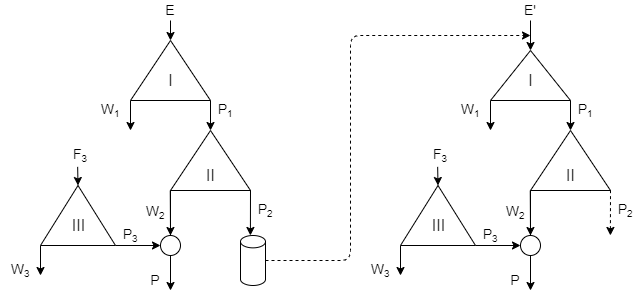
\includegraphics[scale=0.6]{cascades/P2utilizationRing}}
    \caption{Схема передачи загрязненной изотопом $^{232}$U фракции гексафторида урана в двойном каскаде от первой партии дообогащенного регенерированного урана к последующей. Обозначения: $E$ -- поток регенерированного урана; $P_1$ -- поток отбора первого каскада, выступающий питанием второго каскада; $P_2$ -- поток отбора второго каскада; $W_1$ -- поток отвала первого каскада; $W_2$ -- поток тяжелой фракции (условный «отвал») второго каскада; $P_0$ -- поток НОУ-разбавителя; $P$ -- финальный продукт (товарный низкообогащенный уран (НОУ), который подается на питание последующего двойного каскада, перемешиваясь с регенератом очередного рецикла}\label{P2utilizationRing}
\end{figure}

Учитывая, что каскадная схема двойного каскада с НОУ-разбавителем (рис. \ref{p2left}) предназначена для обогащения регенерата с высоким накопившимся в ходе серии пройденых рециклов содержанием изотопа $^{232}$U, можно использовать такую каскадную схему для вовлечения ранее полученного в потоке отбора второго каскада фракции $P_2$ загрязненной изотопом $^{232}$U. Выведенный ранее из системы гексафторида урана может быть перемешан с регенератом, полученным из следующей партии отработавшего топлива, то есть с составом более загрязненным изотопами $^{232,233,234,236}$U, чем исходно использовавшийся состав, побочным продуктом которого оказался этот $P_2$. Полученная таким образом в результате смешения $P_2$ предыдущего рецикла и регенерата очередного рецикла смесь будет отправлена на последующее обогащение (рис. \ref{P2utilizationRing}).

При использовании подобной схемы удастся полностью замкнуть топливный цикл по урану, а единственным отходом производства останется ОГФУ, образующийся в отвале первого каскада, который можно считать штатным отходом обогатительного производства с отработанными технологиями хранения и переработки. При этом после завершения производственного цикла останется невостребованным только тот объем обогащенного по изотопу $^{232}$U гексафторида урана (загрязненной фракции легкого конца второго каскада (рис. \ref{P2utilizationRing})), который будет образован после обогащения последней партии регенерата. Таким образом, предложенный подход к дообогащению регенерата урана позволяет организовать полный возврат регенерированного урана в топливный цикл в течение всего жизненного цикла задействованного урана.

При схожем наборе достоинств и недостатков схемы двойного каскада с НОУ-разбавителем с возвратом потока $P_2$ в цикл (рис. \ref{P2utilizationRing}) с предшественницей, не предусматривающей использование загрязненного потока (рис. \ref{p2left}), достоинством схемы с возвратом $P_2$ является более глубокая выработка потенциала делящегося $^{235}$U, накапливаемого совместно с изотопами $^{232,233,234}$U в загрязненной фракции второго каскада. Это позволяет добиваться меньших потерь $^{235}$U на всем жизненном цикле используемого урана.


\subsubsection{Расчет топливного цикла, осуществляемого посредством двойного каскада с НОУ-разбавителем с возвратом потока $P_2$ в цикл}

Вычислительный эксперимент выполнялся исходя из следующих предположений.

Ординарный каскад, с помощью которого был обогащен регенерат первого рецикла, заменяется для последующих рециклов двойным каскадом ((рис. \ref{p2left}) и  полученная с его помощью партия последующего регенерата, произведенная после дообогащения регенерата первой партии регенерата (или регенерата, выделенного из первой выгруженной группы ТВС из реактора, работающего на РУТ-топливе первого рецикла) фракция, обогащенная по изотопу $^{232}$U и имеющая 20\% содержание изотопа $^{235}$U смешивается с регенератом, полученным после переработки второй партии ОТВС. Полученную смесь направляют на дообогащение (рис. \ref{P2utilizationRing}).


Результаты расчета параметров двойных каскадов для этого случая приведены в табл. \ref{vest2019_2}. В случае, когда возврата потока отбора не происходит, параметры топлива для всех перегрузок второго рецикла совпадают с параметрами первой перегрузки из табл. \ref{vest2019_2}, а изотопный состав урана, попадающего в отходы на каждой перегрузке, и его количество, совпадает с составом возвращаемой фракции первой перегрузки из табл. \ref{vest2019_2}.

\begin{table}
\begin{tabular}{|c|c|c|c|c|c|c|}
    \hline \multicolumn{1}{c|}{ Номер перегрузки } & \multicolumn{2}{|c|}{ Первая перегрузка } & \multicolumn{2}{c|}{ Вторая перегрузка } & \multicolumn{2}{|c}{ Третья перегрузка } \\
    \hline Обогащение, $\%$ & $4.95$ & $4.4$ & $4.95$ & $4.4$ & $4.95$ & $4.4$ \\
    Расх. пр. U, кг & $139802.03$ & $58291.31$ & $135568.06$ & $56351.24$ & $133649.39$ & $56868.39$ \\
    Расх. рег. U, кг & $20604.65$ & $9961.54$ & $20860.12$ & $10082.89$ & $20929.42$ & $10118.12$ \\
    Расх. РР, отн.ед. & $263368.8$ & $109887.15$ & $254313.79$ & $106009.0$ & $252276.2$ & $108260.45$ \\
    Масса $P_2$, кг & $255.47$ & $121.36$ & $324.77$ & $156.59$ & $329.34$ & $220.37$ \\
    \hline
    \end{tabular}
    $C_i$, \%
    \begin{tabular}{c|c|c|c|c|c|c|c}
    \hline${ }^{232} \mathrm{U}$ & $4.43 \times 10^{-7}$ & $4.34 \times 10^{-7}$ & $4.80 \times 10^{-7}$ & $4.85 \times 10^{-7}$ & $5.92 \times 10^{-7}$ & $4.92 \times 10^{-7}$ \\
    ${ }^{233} \mathrm{U}$ & $1.33 \times 10^{-6}$ & $1.32 \times 10^{-6}$ & $1.50 \times 10^{-6}$ & $1.51 \times 10^{-6}$ & $1.74 \times 10^{-6}$ & $1.50 \times 10^{-6}$ \\
    ${ }^{234} \mathrm{U}$ & $5.87 \times 10^{-2}$ & $5.40 \times 10^{-2}$ & $6.14 \times 10^{-2}$ & $5.68 \times 10^{-2}$ & $6.38 \times 10^{-2}$ & $5.63 \times 10^{-2}$ \\
    ${ }^{235} \mathrm{U}$ & $5.154$ & $4.607$ & $5.207$ & $4.658$ & $5.212$ & $4.634$ \\
    ${ }^{236} \mathrm{U}$ & $4.76 \times 10^{-1}$ & $4.91 \times 10^{-1}$ & $6.16 \times 10^{-1}$ & $6.14 \times 10^{-1}$ & $6.22 \times 10^{-1}$ & $5.61 \times 10^{-1}$ \\
    ${ }^{238} \mathrm{U}$ & Остальное & Остальное & Остальное & Остальное & Остальное & Остальное \\
    \hline \multicolumn{4}{|c|}{ Изотопный состав возврашаемой фракции, $\%$}
    \end{tabular}
    % $C_i$, \%
    \begin{tabular}{|c|c|c|c|c|c|c|}
    \hline ${ }^{232} \mathrm{U}$ & $1.64 \times 10^{-5}$ & $1.75 \times 10^{-5}$ & $2.32 \times 10^{-5}$ & $2.36 \times 10^{-5}$ & $2.57 \times 10^{-5}$ & $2.34 \times 10^{-5}$ \\
    ${ }^{233} \mathrm{U}$ & $3.98 \times 10^{-5}$ & $4.17 \times 10^{-5}$ & $5.16 \times 10^{-5}$ & $5.21 \times 10^{-5}$ & $5.49 \times 10^{-5}$ & $5.15 \times 10^{-5}$ \\
    ${ }^{234} \mathrm{U}$ & $5.88 \times 10^{-1}$ & $6.03 \times 10^{-1}$ & $6.78 \times 10^{-1}$ & $6.81 \times 10^{-1}$ & $6.96 \times 10^{-1}$ & $6.73 \times 10^{-1}$ \\
    ${ }^{235} \mathrm{U}$ & $20.00$ & $20.00$ & $20.00$ & $20.00$ & $20.00$ & $20.00$ \\
    ${ }^{236} \mathrm{U}$ & $7.11$ & $7.04$ & $6.54$ & $6.54$ & $6.46$ & $6.55$ \\
    ${ }^{238} \mathrm{U}$ & Остальное & Остальное & Остальное & Остальное & Остальное & Остальное \\
    \hline
    \end{tabular}
    \caption{Изотопные составы и расходы природного урана для изготовления топлива для перегрузок реактора
    типа ВВЭР-1200 (без учета твэгов): топливо второго рецикла. Обозначения: $C_i$ -- изотопный состав возвращаемой фракции; Расх. РР, отн. ед. -- расход работы разделения в относительных единицах; пр. U -- природный уран; рег. U -- урановый регенерат}\label{vest2019_2}
\end{table}


Как видно из данных табл. \ref{vest2019_2} предложенная схема рециклирования действительно позволяет полностью израсходовать и исходный регенерированный уран и образующийся в результате использования двойного каскада высокообогащенный отход.

Итак, опираясь на результаты расчетов, можно сделать общие выводы касаемо двойного каскада с НОУ-разбавителем с возвратом потока $P_2$ в цикл:

\begin{enumerate}
    \item схема принципиально применима для обогащения регенерированного урана в условиях многократного рецикла урана в топливе легководных реакторов, поскольку позволяет получать продукт, отвечающий всем требованиям по концентрациям четных изотопов для регенерата различного исходного состава;
    \item достоинством схемы является полное отсутствие потерь $^{235}$U (не считая потока отвала первого каскада) в процессе рециклирования, а также полное отсутствие нештатного отхода вплоть до последней перегрузки последнего рецикла; Однако, ввиду искусственного повышения содержания четных изотопов $^{232,234}$U в получаемом продукте с каждой последующей перегрузкой возрастает масса отхода  $P_2$ и, соответственно, масса концентрирующегося в нем изотопа $^{235}$U, что уменьшает эффект от возврата изотопа $^{235}$U в цикл из-за его потерь вследствие увеличения потока загрязненной фракции, которое происходит вследствие роста концентраций четных изотопов в исходной смеси.
    \item возврат фракции отхода (потока $P_2$) в схему является причиной монотонного роста концентраций четных изотопов, что приводит к необходимости увеличения уровня обогащения получаемого НОУ и, тем самым, к росту затрат работы разделения, а также повышению концентрации изотопа $^{235}$U в НОУ-разбавителе ввиду необходимости компенсации влияния $^{236}$U;
    \item в схеме присутствуют потери работы разделения из-за необходимости обеднять отбор второго ординарного каскада $P_2$ в последующей составной каскадной схеме;
\end{enumerate}


В качестве общего вывода по результатам анализа схемы двойного каскада с НОУ-разбавителем с возвратом $P_2$ в топливный цикл (рис. \ref{p2left}) представим следующее:
\begin{enumerate}
    \item схема применима для обогащения регенерированного урана в условиях многократного рецикла урана в топливе легководных реакторов, поскольку позволяет получать продукт, отвечающий всем требованиям на концентрации четных изотопов на основе состава регенерата с повышенным исходным содержанием изотопов $^{232,234}$U, который не позволяет решить проблему с помощью ординарного каскада;
    \item схема позволяет использовать поток «легкой» фракции второго каскада ($P_2$), поскольку указанный поток возвращается в топливный цикл, что снимает проблемы его долговременного хранения и связанные с ним затраты;
    \item схема c возвратом $P_2$ как и предшествующая схема без возврата $P_2$, подходит для решения задачи обогащения урана при одновременном выполнении всех сопутствующих условий, в том числе, при обогащении регенерированного урана, прошедшего несколько последовательных рециклов;
    \item схема c возвратом $P_2$ как и предшествующая схема двойного каскада с НОУ-разбавителем, позволяет задействовать для воспроизводства ядерного топлива накопленный в значительных количествах обедненный уран. Производимый ею отвал регенерированного урана ($W_1$) имеет содержание четных изотопов на уровне ниже допустимых ограничений. Это позволяет говорить о том, что такие отвалы могут безопасно длительно хранится в виде гексафторида урана или быть переработанными на установке дефторирования;
    \item в схеме на трех стадиях процесса обогащения происходят потери работы разделения:
    \begin{enumerate}
        \item обеднение отбора первого каскада $P_1$ во втором каскаде;
        \item смешивание потоков $W_2$ с НОУ-разбавителем $P_0$, в которых различается содержание изотопа $^{235}$U;
        \item смешивания потоков $P_2$ и $E$ на входе в каскады, принимающие регенерат последующих рециклов (начиная с третьего).
    \end{enumerate}
    \item в схеме, как и в предшествующей немодифицированной схеме двойного каскада с НОУ-разбавителем, физически разделены участки каскада с разделительным оборудованием, пропускающие через себя регенерированный урана (первые два каскады, принимающие на вход поток $E$ на рисунке \ref{P2utilizationRing}) и участок обогащения сырья для наработки НОУ-разбавителя -- природного или обедненного урана -- материалов, которые не загрязнены четными изотопами $^{232,236}$U. В дальнейшем это позволит задействовать оборудование каскада, использовавшегося для наработки разбавителя, в операциях обогащения природного урана или другого сырьевого материала, не загрязненного четными изотопами, а значит в менее жестконормированных условиях эксплуатации;
    \item практическая реализация представляется нецелесообразной, поскольку данная схема не дает ощутимых преимуществ с точки зрения интегральной экономии $^{235}$U в топливном цикле по отношению к схеме двойного каскада с НОУ-разбавителем (рис. \ref{p2left}), причем реализации схемы с возвратом $P_2$ возможна только в условиях непрерывной работы реактора и постоянного поступления новых партий регенерата на дообогащение.
\end{enumerate}


\section{Схема тройного каскада с НОУ-разбавителем и дополнительным разбавителем потока $P_2$, возвращаемого в цикл}

Другим вариантом модификации каскадной схемы, представленной на (рис. \ref{p2left}) стала схема тройного каскада \cite{smirnovApplyingEnrichmentCapacities2018}. Принцип ее работы, наследуя заложенные в предшествующих схемах идеи, состоит в следующем дополнении.

\begin{figure}[ht]
    \centerfloat{
\includegraphics[scale=0.9]{cascades/p2_withDepU}}
    \caption{Тройной каскад для обогащения регенерированного урана. Обозначения: $E$ -- поток регенерированного урана; $P_1$ -- поток отбора первого каскада, выступающий питанием второго каскада; $P_2$ -- поток отбора второго каскада; $F_{du}$ -- поток ОГФУ-разбавителя, смешиваемого с $P_2$ перед подачей на вход третьего каскада; $W_1$ -- поток отвала первого каскада; $W_2$ -- поток тяжелой фракции (условный «отвал») второго каскада; $P_0$ -- поток НОУ-разбавителя; $P$ -- финальный продукт (товарный низкообогащенный уран (НОУ)), полученный смешиванием потоков $W_2$, $P_0$ и $P_3$, где $P_3$ -- отбор третьего каскада; $W_3$ -- отвал третьего каскада.}\label{p2_withDepU}
\end{figure}

В реализации такой схемы поток легкой фракции второго каскада $P_2$ перемешивается со складским ОГФУ и направляется на последующее обогащение в третий каскад (рис. \ref{p2_withDepU}). Пропорцию смешивания $P_2$ с ОГФУ определяют исходя из возможности получить НОУ надлежащего качества при обогащении их смеси (оставаясь в рамках ограничений по четным изотопам). Остальные параметры схемы тройного каскада следует подбирать исходя из того, что финальный продукт будет получен смешиванием трех потоков: низкообогащенного <<чистого>> разбавителя $P_0$, тяжелой <<очищенной>> фракции $W_2$ второго каскада и, полученного при обогащении потока $P_2$ и обедненного урана, изотопного состава $P_3$. Управляющими параметрами являются: концентрации на выходах $P_1$ первого и $P_2$ второго каскадов, а также в потоке НОУ-разбавителя $P_0$. При детерминированной их комбинации обеспечивается соответствие предзаданному отношению масс конечного продукта и исходного регенерата, за счет чего выполняется условие полного возврата. При этом проблема высокоактивного отхода решается без выхода за пределы концентрации допустимой для обогащения регенерата (20\%). Также устраняется необходимость обращения с $P_2$, которое в схеме двойного каскада с НОУ-разбавителем с возвратом потока $P_2$ в цикл (рис. \ref{P2utilizationRing}) связано с его отложенным вовлечением из-за зависисмости от последующих поступлений на обогащение новых партий (последующих рециклов) регенерата.

Таким образом, решение проблемы накопления нештатного отхода, характерной для двойного каскада с НОУ-разбавителем, состоит в том, что поток легкой фракции второго каскада ($P_2$) перемешивают с обедненным ураном и направляют на последующее обогащение в еще один каскад (крайний правый каскад на рисунке \ref{p2_withDepU}).

Для анализа возможностей схемы двойного каскада с НОУ-разбавителем, представим расчет оценивающий издержки ее применения для возврата регенерата пятого рецикла. 
В качестве ключевых оцениваемых характеристик будем опираться на экономию природного урана, а также долю дополнительно задействуемых в каскаде центрифуг, по сравнению с ординарным каскадом для обогащения природного урана. Проведем сравнение со схемой с разбавлением регенерата природным ураном перед подачей в ординарный трехпоточный каскад \ref{o3} \cite{smirnovMethodEnrichReprocessed2019}. Обе сравниваемые схемы должны обеспечить производство НОУ коммерческого качества, то есть удовлетворяющего всем заданным условиям.

В таблице \ref{tr_ch} представлены величина экономии природного урана, потребление регенерированного урана на единицу продукта, а также количество центрифуг для предложенной трехкаскадной схемы и модифицированного ординарного каскада, по сравнению с базовым вариантом -- ординарным  каскадом, обогащающим природный уран. Количество центрифуг для всех вариантов приводится к количеству центрифуг в ординарном каскаде для обогащения природного урана.

\begin{table}[h]
\centering
\normalsize\begin{tabulary}{1.0\textwidth}{CCCCCCC}
    Каскад & Экономия природного урана, \% & Доп. разделительные мощности, \% & Расход регенерата на ед. продукта \\
    Ординарный модифицированный & 7.1 & 3.6 & 49.2 \\
        &  &  &   \\
    Двойной каскад с НОУ-разбавителем & 38.3 & 97.3 &  92.4 \\
        &  &  &   \\
\end{tabulary}
\caption{{Оцениваемые параметры рассматриваемых схем{\label{tr_ch}}}}
\end{table}

В табл. \ref{tr_prod} показан изотопный состав НОУ коммерческого уровня, полученного в предлагаемом тройном каскаде.

\begin{table}[h]
    \centering
    \normalsize\begin{tabulary}{1.0\textwidth}{ccccccc}
        Массовое число & 232 & 233 & 234 & 235 & 236 \\
        C, \% & 5.00e-7 & 6.88e-7 & 5.31e-2 & 5.11 & 0.57 \\
    \end{tabulary}
    \caption{{Изотопный состав НОУ-продукта схемы двойного каскада с НОУ-разбавителем и дополнительным разбавителем потока $P_2$, возвращаемого в цикл{\label{tr_prod}}}}
    \end{table}

Эти результаты показывают, что предложенная схема решает поставленную в диссертации задачу. Сравнение с ординарным каскадом показывает, что даже при выбранном «грязном» составе регенерированного урана -- составе пятого рецикла -- можно сэкономить более трети природного урана, что намного больше, чем достижимо при использовании простых модификаций. Однако, такие преимущества влекут за собой увеличение затрат разделительной работы, а следовательно, и количества центрифуг примерно на 97\% по сравнению с ординарным трехпоточным каскадом, который обогащает природный уран. Схема также позволяет производить НОУ товарного качества, расходуя заранее определенное количество переработанного урана без нежелательных нештатных побочных продуктов, за исключением стандартных т.н. хвостов разделительного производства (потоков отходов) разделительных каскадов в виде обедненного урана.

Рассчитывая материальные балансы в этой схеме, исходя из предположения, что будет произведена ровно 21 тонна НОУ. Примерно такая масса урана требуется для загрузки реактора ВВЭР-1200 твэлами с обогащением 4,95\%. Имея заданное отношение регенерата к конечному продукте 0,93, регенерированный уран будет израсходован из расчета 19,53 тонны на 21 тонну конечного продукта НОУ. В нашем случае первый каскад производит 17,5 т обедненного урана в потоке $W_1$, что дает $\approx$2,03 т $P_1$ с концентрацией $^{235}$U, равной 9,41\%. Поток $P_1$ запитывает второй каскад, который, в свою очередь, производит «очищенную» смесь $W_2$ (1,7 тонны, которая содержит 7,34\% $^{235}$U) и загрязненный $P_2$ ($\approx$332 кг), который содержит 20\% $^{235}$U. $P_2$ поступает в третий каскад и там разбавляется 3298,88 т. обедненного урана с концентрацией $^{235}$U 0,1\%. В третьем каскаде обедняющая часть состоит всего из 1 ступени, выдает $\approx$3293,1 тонны отходов $W_3$  с 0,093\% $^{235}$U. НОУ-разбавитель $P_0$ $\approx$13,2 тонны смешивается с 1,7 тоннами $W_2$, образуя $\approx$14,9 тонны материала, которые затем, смешавшись с 6,1 тонны $P_3$, образуют 21 тонну конечного НОУ-продукта. Каскад, производящий НОУ-разбавитель $P_0$ (с концентрацией $^{235}$U 4,9\%), потребляет $\approx$103,6 тонны природного урана, отправляя в отвал $W_0$ 90,4 тонны (с концентрацией 0,1\% $^{235}$U). В результате схема производит (90,4 + 17,5 + 3293) $\approx$3401 тонну обедненного урана. При этом на схему уходит $\approx$3300 тонн складских запасов обедненного урана. Следовательно, фактический выход обедненного урана составляет $\approx$100 тонн, при том что ординарный каскад для обогащения природного урана при производстве такого же количества продукта (21 тонна) производит $\approx$146 тонн, то есть схема тройного каскада с НОУ-разбавителем и дополнительным разбавителем потока $P_2$, возвращаемого в цикл позволяет в полтора раза уменьшить накопление ОГФУ.

Также была предложена реализация поставленной задачи с помощью рассматриваемой схемы, в \cite{gusevMultycascadeEnrichmentSchemes2020}, демонстрирующей споcоб решения задачи возврата регенерата в цикл для состава пятого рецикла при заданной пропорции регенерата к конечному продукту, соответствующей использованию всего выделенного из ОЯТ урана, а также исключающий накопление нештатного отхода за счет разбавления $P_2$ обедненным гексафторидом с последующим обогащением. Как показывают результаты анализа повторного обогащения регенерата пятого рецикла с помощью такой схемы, осуществлять такую операцию можно с различными показателями затрат работы разделения, экономии природного урана, а также вовлечения ОГФУ. Например, ценой расхода дополнительных $\approx$25\% работы разделения, удается вернуть заданное количество переработанного урана, прошедшего пятикратное (5 топливных кампаний) облучение, сэкономив $\approx$15\% природного урана, при этом вовлекая в производство единицы конечного продукта $\approx$31 единицы смеси обедненного урана. Для экономии же природного урана на уровне $\approx$23\%, необходимо, использовав $\approx$74,5 единиц ОГФУ на единицу продукта, допустив перерасход работы разделения на уровне $\approx$50\%. Показатели приведены в соотношении с аналогичными для схемы ординарного каскада для обогащения природного урана, получающего на выходах в продукте и отвале такие же концентрации $^{235}$U (соответствующую $C_{235 экв.}$ в продукте).


Стоит отметить, что представленные примеры приведены только в иллюстративных целях. Чтобы применить эту схему на практике, в первую очередь необходимо оптимизировать ее по выбранному критерию эффективности.

Рассматривая возможность постановки оптимизационной задачи для тройного каскада, в качестве управляющих оптимизационных переменных можно рассматривать: концентрации $^{235}$U в потоках $P_1$, $P_2$ и $W_3$ и отношение потоков $F_{du}$/$P_2$.
Цель решения оптимизационной задачи: при заданных внешних условиях и выполнении заданных ограничений определить наилучшее значение критерия эффективности -- суммарного потока каскадной схемы, в зависимости от варьируемых переменных.

Также, помимо минимума суммарного потока, оптимизационным критерием может выступать минимизация расхода природного урана, а также максимум суммарной степени извлечения $^{235}$U в схеме \ref{Rec3} и из регенерата \ref{RecR3} для тройного каскада, где $RepU$ -- это поток регенерата, а $DepU_{3}$ -- поток разбавляющего $P_2$ ОГФУ.


\begin{equation} \label{Rec3} 
    U^{235}_{Rec} = \frac{LEU Product \cdot C_np}{F_0 \cdot C_{NatU}^{235} + RepU \cdot C_{RepU}^{235} + {DepU}_3 \cdot C_{DepU}^{235}}, 
\end{equation} 
\begin{equation} \label{RecR3} 
    RepU^{235}_{Rec} = \frac{W_2\cdot C_{W_2}^{235}+P_3\cdot C_{P_3}^{235}\cdot \frac{P_2\cdot C_{P_2}^{235}}{P_2\cdot C_{P_2}^{235}+ {DepU}_3 \cdot C_{DepU}^{235}}}{RepU \cdot C_{RepU}^{235}}        
\end{equation} 

Такой тип оптимизационной задачи также как и для предыдущих составных схем представляет собой задачу условной оптимизации функции многих переменных. В диссертационной работе предложена оригинальная методика, основанная на использовании современных методов условной оптимизации и реализованная в виде разработанного в НИЯУ МИФИ программного кода.

% Для такого расчета расчета и оптимизации схемы 3 предложена оригинальная методика, основанная на использовании современных методов условной оптимизации и реализованная в виде разработанного в НИЯУ МИФИ программного кода.

% Следует отметить, что в литературе по данной тематике отсутствуют методики оптимизации трех- и четырехкаскадных схем в случае разделения многокомпонентных смесей. Фактически подобные задачи решены впервые.

Как результат, схема тройного каскада с НОУ-разбавителем и дополнительным разбавителем потока $P_2$, возвращаемого в цикл, позволяя в полноте решить поставленную задачу, не оставляет никакого нештатного отхода, требующего особых мер обращения. В конечном итоге образуется только штатный отход в виде отвалов $W_1$ и $W_3$ , процедуры обращения с которыми на разделительном производстве технологически отработаны. Если получить их смешением ($W_1$ и $W_3$) обедненный уран, он будет содержать изотопы $^{232,234}$U в количествах в десятки/сотни раз сниженных, относительно исходного регенерата. Следовательно, полученный в такой схеме обедненный уран может быть переведен в двуокись урана, например, при помощи установки «W-ЭХЗ». Отсутствие нештатных отходов, загрязненных четными изотопами и является отличительным достоинством рассмотренной схемы, тогда как недостатком выступают дополнительные потери работы разделения, возникающие при перемешивании потока $P_2$ и подмешиваемого к нему в качестве разбавителя ОГФУ.

\subsubsection{Оптимизация схемы тройного каскада с НОУ-разбавителем при различных критериях}

\begin{table}
    \begin{tabular}{cccc}
        $\text{Параметр | Критерий оптимизации}$ & $\text{1}$ & $\text{2}$ & $\text{3}$\\ \hline
        $\text{Интегральная степень извлечения}$ & $0.8684$ & $0.502$ & $0.3692$\\ \hline$\text{Степень извлечения из регенерата}$ & $0.8261$ & $0.9276$ & $0.9179$\\ \hline
        $\text{Расход природного урана на ед. продукта}$ & $6.402$ & $1.172$ & $6.246$\\ \hline$\text{Потери работы разделения}$ & $-2.604$ & $171.0$ & $-4.835$\\ \hline
        $\text{CnP0, \%}$ & $4.125$ & $7.383$ & $4.783$\\ \hline
        $\text{CnP1, \%}$ & $41.0$ & $5.0$ & $7.0$\\ \hline
        $\text{CnP2, \%}$ & $52.0$ & $78.64$ & $54.0$\\ \hline$\text{Р2 на ед. продукта}$ & $0.002729$ & $0.0006247$ & $0.00063$\\ \hline
        $\text{Mk1}$ & $238$ & $238$ & $238$\\ \hline
        $\text{Mk2}$ & $232$ & $232$ & $232$\\ \hline
        $\text{U-232, \%}$ & $5.0e-7$ & $4.768e-7$ & $5.0e-7$\\ \hline
        $\text{U-234, \%}$ & $0.05937$ & $0.04463$ & $0.061$\\ \hline
        $\text{U-235, \%}$ & $5.109$ & $5.162$ & $5.154$\\ \hline
        $\text{U-236, \%}$ & $0.5478$ & $0.7389$ & $0.7044$
    \end{tabular}
\caption{Параметры схемы двойного каскада с НОУ-разбавителем при различных критериях оптимизации.{\label{5opt2}}}
\end{table}


\begin{table}
    \begin{tabular}{cccc}
        $\text{Параметр | Критерий оптимизации}$ & $\text{1}$ & $\text{2}$ & $\text{3}$\\ \hline
        $\text{Интегральная степень извлечения}$ & $0.852$ & $0.6489$ & $0.8164$\\ \hline
        $\text{Степень извлечения из регенерата}$ & $0.8779$ & $0.9129$ & $0.8682$\\ \hline
        $\text{Расход природного урана на ед. продукта}$ & $6.845$ & $6.933$ & $6.377$\\ \hline
        $\text{Потери работы разделения}$ & $4.674$ & $3.09$ & $-0.9778$\\ \hline
        $\text{CnP0, \%}$ & $4.428$ & $5.308$ & $4.95$\\ \hline
        $\text{CnP1, \%}$ & $35.0$ & $5.0$ & $5.0$\\ \hline
        $\text{CnP2, \%}$ & $74.99$ & $72.16$ & $67.98$\\ \hline
        $\text{Р2 на ед. продукта}$ & $0.0004965$ & $0.0001653$ & $0.0009429$\\ \hline
        $\text{Mk1}$ & $238$ & $238$ & $238$\\ \hline
        $\text{Mk2}$ & $232$ & $232$ & $232$\\ \hline
        $\text{U-232, \%}$ & $5.0e-7$ & $5.0e-7$ & $3.21e-7$\\ \hline
        $\text{U-234, \%}$ & $0.06638$ & $0.06911$ & $0.05963$\\ \hline
        $\text{U-235, \%}$ & $5.185$ & $5.24$ & $4.9$\\ \hline
        $\text{U-236, \%}$ & $0.8118$ & $0.9984$ & $0.9883$
    \end{tabular}
\caption{Параметры схемы двойного каскада с НОУ-разбавителем при различных критериях оптимизации.{\label{5opt5}}}
\end{table}


Для демонстрации возможностей, получаемых применением предложенных в диссертации методик оптимизации, представим серию расчетов двойного каскада с НОУ-разбавителем, получив интегральные показатели для различных оптимизационных критериев.

В расчетах оптимальные значения для ключевых параметров достигались при условии несмешивания по относительной концентрации компонентов $^{235}UF_6$ к $^{236}UF_6$ в первом и вотором каскаде схемы.

Критерии оптимизации 1 -- максимум интегральной степени извлечения схемы; 2 -- максимум степени извлечения из регенерата; 3 -- потери работы разделения.

\begin{table}
    \begin{tabular}{cccc}
        $\text{Параметр | Критерий оптимизации}$ & $\text{1}$ & $\text{2}$ & $\text{3}$\\ \hline
        $\text{Интегральная степень извлечения}$ & $0.7271$ & $0.06591$ & $0.06591$\\ \hline
        $\text{Степень извлечения из регенерата}$ & $0.8088$ & $0.8569$ & $0.8569$\\ \hline
        $\text{Расход природного урана на ед. продукта}$ & $6.194$ & $6.219$ & $6.219$\\ \hline
        $\text{Потери работы разделения}$ & $4.17$ & $-0.3242$ & $-0.3242$\\ \hline
        $\text{CnP0, \%}$ & $4.499$ & $4.606$ & $4.606$\\ \hline
        $\text{CnP1, \%}$ & $11.0$ & $9.0$ & $9.0$\\ \hline
        $\text{CnP2, \%}$ & $20.0$ & $20.0$ & $20.0$\\ \hline
        $\text{Р2 на ед. продукта}$ & $0.009947$ & $0.005553$ & $0.005553$\\ \hline
        $\text{Mk1}$ & $238$ & $238$ & $238$\\ \hline
        $\text{Mk2}$ & $232$ & $232$ & $232$\\ \hline
        $\text{U-232, \%}$ & $5.0e-7$ & $5.0e-7$ & $5.0e-7$\\ \hline
        $\text{U-234, \%}$ & $0.05842$ & $0.05949$ & $0.05949$\\ \hline
        $\text{U-235, \%}$ & $5.124$ & $5.138$ & $5.138$\\ \hline
        $\text{U-236, \%}$ & $0.5984$ & $0.6472$ & $0.6472$
        \end{tabular}
\caption{Параметры схемы двойного каскада с НОУ-разбавителем при различных критериях оптимизации.{\label{5opt2_20}}}
\end{table}

\begin{table}
    \begin{tabular}{cccc}
        $\text{Параметр | Критерий оптимизации}$ & $\text{1}$ & $\text{2}$ & $\text{3}$\\ \hline
        $\text{Интегральная степень извлечения}$ & $0.5705$ & $0.04207$ & $0.04207$\\ \hline
        $\text{Степень извлечения из регенерата}$ & $0.6908$ & $0.7376$ & $0.7376$\\ \hline
        $\text{Расход природного урана на ед. продукта}$ & $6.729$ & $6.854$ & $6.854$\\ \hline
        $\text{Потери работы разделения}$ & $18.26$ & $12.25$ & $12.25$\\ \hline
        $\text{CnP0, \%}$ & $5.162$ & $5.081$ & $5.081$\\ \hline
        $\text{CnP1, \%}$ & $7.0$ & $7.0$ & $7.0$\\ \hline
        $\text{CnP2, \%}$ & $20.0$ & $20.0$ & $20.0$\\ \hline
        $\text{Р2 на ед. продукта}$ & $0.01248$ & $0.00904$ & $0.00904$\\ \hline
        $\text{Mk1}$ & $238$ & $238$ & $238$\\ \hline
        $\text{Mk2}$ & $232$ & $232$ & $232$\\ \hline
        $\text{U-232, \%}$ & $5.0e-7$ & $5.0e-7$ & $5.0e-7$\\ \hline
        $\text{U-234, \%}$ & $0.06017$ & $0.06215$ & $0.06215$\\ \hline
        $\text{U-235, \%}$ & $5.179$ & $5.191$ & $5.191$\\ \hline
        $\text{U-236, \%}$ & $0.7908$ & $0.832$ & $0.832$
        \end{tabular}
\caption{Параметры схемы двойного каскада с НОУ-разбавителем при различных критериях оптимизации.{\label{5opt5_20}}}
\end{table}

В качестве итогового списка характеристических особенностей схемы тройного каскада следует обозначить следующие:

\begin{enumerate}
    \item применима для обогащения регенерированного урана в условиях многократного рецикла и позволяет получать продукт, отвечающий всем требованиям по концентрациям четных изотопов для регенерата различного исходного состава как показано на рассматриваемых входных изотопных составах;
    \item достоинством схемы является полное отсутствие нештатных отходов, требующих специального обращения, поскольку на выходе из схемы, помимо основного продукта, возникают только потоки обедненного урана в виде отвалов каскадов схемы. Причем, в отличие от схемы двойного каскада с НОУ-разбавителем, отход отсутствует при любом варианте использования: как для однократного обогащения регенерированного урана, так и в условиях постоянных поступлений партий регенерированного урана последовательных перегрузок реактора;
    \item как и предшествующие схемы, схема позволяет задействовать для воспроизводства ядерного топлива накопленный в значительных количествах обедненный уран;
    \item в схеме отделены участки обогащения регенерированного урана и участок обогащения обедненного или природного урана (каскад, расположенный на схеме слева (рис. 
    \ref{p2_withDepU})), не загрязненного четными изотопами. В дальнейшем это позволит использовать оборудование этого каскада для обогащения природного урана или другого сырьевого материала, не загрязненного четными изотопами;
    \item получаемый в схеме отвал регенерированного урана в потока $W_1$ и $W_3$ имеет содержание изотопа $^{232}$U ниже, чем исходный регенерат. Подобный материал можно длительно хранить или отправить на переработку в установке дефторирования. В случае же необходимости дополнительного понижения концентраций четных изотопов данный поток может быть дополнительно разбавлен конечными отвалами с обогащением ниже 0,13\%. 
    \item недостатком схемы являются потери работы разделения из-за необходимости:
    \begin{enumerate}
        \item обеднять отбор первого каскада в последующем втором каскаде;
        \item смешивание потоков $W_2$ с НОУ-разбавителем $P_0$, а затем и с $P_3$ в которых различается содержание изотопа $^{235}$U;
        \item смешивания потоков $P_2$ и $F_{du}$ на входе в третий каскад.
    \end{enumerate}
\end{enumerate}


% Слабое изменение параметров каскадной схемы в условиях многократного рецикла позволяет говорить о возможности «настройки» данной каскадной схемы на возможность работы с регенератом различных рециклов при минимальных изменениях параметров. В частности, для данной схемы возможно подобрать «унифицированный» разбавитель с фиксированным содержанием 235U, что могло бы позволить не привязывать напрямую мощности по получению разбавителя из обедненного урана (каскад 3) к каскадам, работающим с регенератом. Иными словами, в этом случае разбавитель мог бы нарабатываться независимо от поступлений конкретных партий регенерата.


\section{Схема независимой утилизации побочного продукта легкой фракции второго каскада схемы двойного каскада с НОУ-разбавителем}

В диссертационной работе предложен способ обращения с $P_2$, который позволяет вовлечь выведенный из системы схемой двойного каскада с НОУ-разбавителем изотоп (рис. \ref{p2left}) $^{235}$U. Предлагаемая схема направлена на решение следующих задач.

\begin{enumerate}
  \item Сокращение доли потребляемого обедненного урана при сохранении возможности использования высокообогащенного побочного продукта;
  \item Обеспечение полного возврата регенерированного урана в топливный цикл;
  \item Повышение эффективности использования делящегося изотопа $^{235}$U из регенерата;
  \item Увеличение экономии природного урана на производство единицы свежего топлива для загрузки легководного реактора.
\end{enumerate}

Принцип схемы, изображенной на рис. \ref{P2utilization}, представляющей из себя модификацию схемы двойного каскада с НОУ-разбавителей (рис. \ref{p2left}) состоит в следующем.
Образовавшаяся на легком конце второго каскада изотопная легкая фракция $P_2$  разбавляется потоком складского ОГФУ ($F_{du}$) до такого уровня $^{235}$U в их смеси, который соответствует концентрации $^{235}$U в потоке дополнительного разбавителя в виду низкообогащенного урана ($F_{leu}$), изготавливаемого из из природного урана. необходимого в продукте, с добавкой, которая учитывает компенсацию $^{236}$U. Пропорцию этого НОУ-разбавителя подбирают таким образом, чтобы при обогащении полученной из этих трех компонентов смеси в ординарном каскаде, при достижении обогащаемой смесью на легком конце каскада (в  $P_{add}$) концентрации $^{235}$U требуемой в конечном НОУ-продукте, рассчитываемой с поправкой на компенсацию $^{236}$U, достигалось соответствие содержания $^{232}$U заданному предельному значению.

\begin{figure}[ht]
  \centerfloat{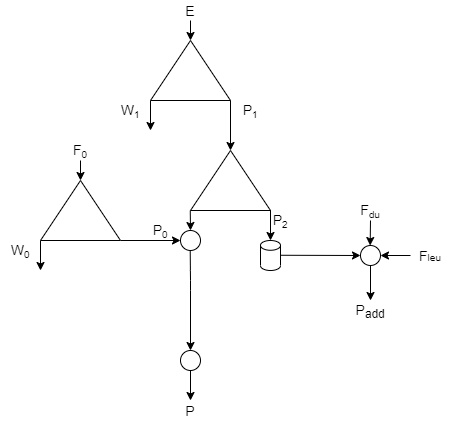
\includegraphics[scale=0.7]{cascades/P2utilization}}
  \caption{Схема независимого вовлечения загрязненногой изотопом $^{232}$U фракции с разбавлением обедненным и природным ураном}\label{P2utilization}
\end{figure}

Расчет целевых показателей схемы -- доли дополнительного НОУ-продукта, полученного из $P_2$, от новой ТВС (469 кг), а также экономии природного урана, производился на основе данных составов второго и пятого рециклов (см.постановку задачи), а также предположения двукратного увеличения предела содержания $^{232}$U в продукте, дополнительно произведенном из $P_2$ ($1\cdot10^{-7}$\% вместо $5\cdot10^{-7}$\%). Результаты вычислений представлены в таблице \ref{independent}.


\begin{table}[h]
  \centering
  \normalsize\begin{tabulary}{1.0\textwidth}{CCCCC}
  ПДК $^{232}$U & Цикл № & $P_2$, кг & Дополнительный продукт из $P_2$, доля новой ТВС, \% & Экономия природного урана, \% \\
  1.e-6\% & 2 & 1.09 & 7.11 & 14.6 \\
   & 5 & 0.92 & 10.21 & 6.3 \\
  5.e-7\% & 2 & 1.33 & 14.22 & 7.3 \\
   & 5 & 0.92 & 20.42 & 3.1 \\
  \end{tabulary}
  \caption{Результаты вовлечения $P_2$ в производство дополнительного НОУ-продукта. Обозначения: ПДК $^{232}$U -- предельно допустимая концентрация $^{232}$U в дополнительно производимом на основе $P_2$ продукте. {\label{independent}}}
\end{table}

Проведем анализ численных результатов расчета. Значения в столбце <<Дополнительный продукт из $P_2$, доля новой ТВС \%>> соответствуют доле дополнительно произведенного НОУ из побочного $P_2$, образовавшегося в процессе обогащения топлива из регенерата для одной ТВС (469 кг), а экономия природного урана приведена относительно схемы ординарного каскада для обогащения природного урана.

Как можно заключить из результатов, представленных в таблице \ref{independent}, предлагаемый способ использования $P_2$ через модификацию схемы двойного каскада с НОУ-разбавителем позволяет экономить дополнительное количество природного урана относительно двойного модифицированного каскада, в котором не предполагается задействование потока легкой фракции второго каскада. А эффект более значителен для случаев, когда задействуется побочный продукт $P_2$ двойного каскада, образующийся на начальных стадиях рециклирования уранового топлива. В рассматриваемом случае -- это второй рецикл (табл. \ref{independent}). Схема рис. \ref{P2utilization} также показывает себя как более предпочтительная в экономии природного урана (вдвое выигрышнее, согласно табл. \ref{independent}), когда предельно допустимая концентрация $^{232}$U в получаемом из $P_2$ конечном продукте допускается на уровне в два раза выше ($1\cdot10^{-7}$\% вместо $5\cdot10^{-7}$\%).  Значение экономии природного урана соответствует доле $P_2$, смешанной с обедненным ураном $F_{du}$, до того, как он будет смешан с НОУ-разбавителем $F_{leu}$, полученным из природного урана. Важно заметить, что значение этой доли соответствует экономии работы разделения, которая, в случае отказа от использования $P_2$, была бы затрачена на прямое обогащение природного урана в ординарном каскада для производства аналогичного замещающего количества свежего НОУ-продукта.

Итак, накопленный в ходе производства одной ТВС из регенерата побочный продукт $P_2$ можно использовать для производства дополнительных $\approx$7\% свежего НОУ-продукта от дополнительной топливной сборки. Это соответствует возможности произвести дополнительную 15-ю тепловыделяющую сборку из накопленного $P_2$, образовавшегося при производстве предыдущих четырнадцати ТВС. Таким образом, для современного легководного реактора, такого как, например, российский ВВЭР-1200 или европейский PWR, где активная зона состоит из более чем 150 тепловыделяющих сборок, взяв за основу предложенную схему, можно изготовить дополнительно более 10 ТВС. 



В качестве выводов, относящихся ко всем рассмотренным схемам, приведем следующие:
\begin{enumerate}
    \item схемы на основе двойного каскада, использующие НОУ-разбавитель, принципиально пригодны для решения задачи обогащения регенерированного урана в рамках многократного рецикла урановой составляющей топлива легководных реакторов. При этом каждая из схем имеет собственные достоинства и недостатки;
    \item характерным недостатком схемы, не предполагающей утилизацию нештатного отхода, образующегося в потоке $P_2$, является проблема с обращением с этим материалом, с высоким содержанием как четных изотопов (на 1-2 порядка выше, чем пределы для товарного НОУ) и $^{235}$U (до 20\% или, в некоторых случаях, до 90\%, в зависимости от выбранного режима работы каскадной схемы). Одним из вариантом обращения с ним, помимо схемы независимой утилизации побочного продукта легкой фракции второго каскада схемы двойного каскада с НОУ-разбавителем (рис. \ref{P2utilization}), может стать его перемешивание с отвалом первого каскада при обогащении регенерата. Оценки показали, что в этом случае возможно получить обедненный уран с приемлемым содержанием $^{232}$U (не выше $5\cdot10^{-7}$\%);
    \item характерными недостатком схемы двойного каскада с НОУ-разбавителем с возвратом потока $P_2$ в цикл (рис. \ref{P2utilizationRing}) является возврат значительной части четных изотопов на вход каскадной схемы;
    \item характерным недостатком схемы тройного каскада (рис. \ref{p2_withDepU}) являются дополнительные затраты работы разделения по отношению к схемам двойного каскада с НОУ-разбавителем, возникающие при обогащении разбавленного обедненным ураном отхода второго каскада схемы, загрязненного четными изотопами.
  \end{enumerate}

Анализ эффективности предложенных каскадных схем с точки зрения потерь $^{235}$U показал, что перспективными вариантами для дальнейшей технико-экономической проработки являются каскадные схемы двойного каскада с НОУ-разбавителем (рис. \ref{p2left}) и тройного каскада (рис. \ref{p2_withDepU}). Cхема двойного каскада с НОУ-разбавителем на каждом из рассмотренных рециклах позволяет извлечь более 80\% от массы $^{235}$U из исходного регенерированного урана, поступившего на обогащение.

Для каждой из предложенных схем разработаны оригинальные методики расчета и оптимизации ее переменных по критерию минимума суммарного потока каскадной схемы, основанная на использовании современных методов условной оптимизации функций многих переменных. С использованием разработанных методик расчета и оптимизации предложенных каскадных схем продемонстрирована возможность их использования для обогащения регенерированного урана в условиях многократного рецикла на примере взятого из литературы изотопного состава регенерата урана с повышенным содержанием четных изотопов и отвечающего пятому рециклу в топливе ВВЭР.

Для выбора конкретного варианта каскадной схемы для организации производственного процесса, необходим детальный технико-экономический анализ каждой из схем на основе их интегральных показателей, таких как расход сырьевых материалов и работы разделения, в контексте всей цепочки ядерного топливного цикла, а также с учетом возникающих в этой цепочке изменений при использовании регенерата урана по отношению к открытому топливному циклу. Помимо этого, необходима проработка технологических проблем каждой из схем, в частности, с точки зрения возможности эксплуатации и обслуживания оборудования в условиях работы с материалами, имеющими более высокую, чем природный уран удельную активность. Например, подобные условия возникают в каскадах, концентрирующие в легкой фракции $\alpha$-активные изотопы $^{232,234}$U. 



\clearpage